% This work is licensed under the Creative Commons Attribution-NonCommercial-NoDerivs
% 3.0 Unported License. To view a copy of this license, visit
% http://creativecommons.org/licenses/by-nc-nd/3.0/ or send a letter to
% Creative Commons, 444 Castro Street, Suite 900, Mountain View, California, 94041, USA.

%-------------------------------------------------------------------------------
\begin{frame}\frametitle{Résumé des principales commandes}
  cheatsheet: \url{https://github.com/AlexZeitler/gitcheatsheet}
\end{frame}
%-------------------------------------------------------------------------------
\begin{frame}[fragile]\frametitle{Création}

% TODO : faire en // la manip sur un terminal
  \begin{block}{À partir de fichiers locaux}
    \begin{semiverbatim}
\$ \alert{git init}
    \end{semiverbatim}
  \end{block}
  \begin{block}{À partir d'un dépôt existant}
    \begin{semiverbatim}
\$ \alert{git clone git@github.com:excilys/formation-git.git}
    \end{semiverbatim}
  \end{block}

\end{frame}
%-------------------------------------------------------------------------------
\begin{frame}[fragile]\frametitle{Anatomie d'un projet git}
  \begin{semiverbatim}
  \$ \alert{ls -A1}
  formation.tex
  \alert{.git/}
  .gitignore
  images/
  Makefile
  \end{semiverbatim}

  Le .git représente le dépôt git, il contient l'ensemble des
  commits, branches et tags créés.
\end{frame}
%-------------------------------------------------------------------------------
\begin{frame}[fragile]\frametitle{Le fichier .gitignore}
  chemins (fichiers et/ou dossiers) ignorés par git
  \begin{semiverbatim}
  \$ \alert{cat .gitignore}
  .project
  target
  *.iml
  *.ipr
  *.iws
  *.idea
  \end{semiverbatim}

\end{frame}
%-------------------------------------------------------------------------------
\begin{frame}[fragile]\frametitle{Visualisation}
  Historique des commits: \verb|git log|

  \begin{semiverbatim}
  \$ \alert{git log}
  \end{semiverbatim}


  Auteurs des dernières modifications: \alert{git blame}
\end{frame}
%-------------------------------------------------------------------------------
\begin{frame}\frametitle{Staging area (ou Stage)}
  Zone intermédiaire entre l'espace de travail et le dépôt
  \begin{center}
    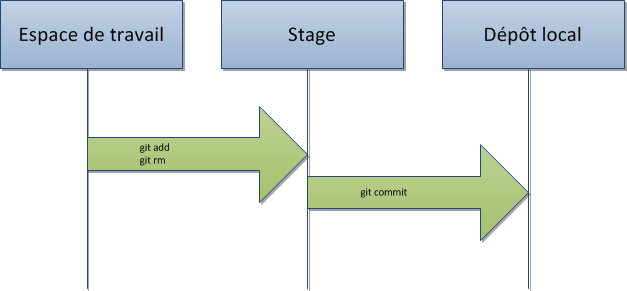
\includegraphics[width=\textwidth]{./images/staging-area.png}
  \end{center}

\end{frame}
%-------------------------------------------------------------------------------
\begin{frame}[fragile]\frametitle{Manipuler la staging area}
  \begin{itemize}
    \item \alert{git add} : ajoute ("stage") un fichier à la staging area
    \item \alert{git rm} : supprime un fichier managé et enregistre sa suppression
      dans la staging area
    \item \alert{git reset HEAD} : retire des modifications de la staging area
  \end{itemize}

  \textit{bonus : git add -p, git add -A}

\end{frame}
%-------------------------------------------------------------------------------
\begin{frame}[fragile]\frametitle{Visualisation}

\begin{semiverbatim}

  \$ \alert{git status}
  # On branch master
  #
  # Changes to be committed:
  #
  modified: some_text.txt \alert{ <-- modifié puis staged}
  #
  # Changes not staged for commit:
  #
  modified: some_more_text.txt \alert{ <-- modifié, non staged}
  #
  \end{semiverbatim}
\end{frame}
  
%-------------------------------------------------------------------------------
\begin{frame}[fragile]\frametitle{Visualisation}
  
\begin{semiverbatim}

  \$ \alert{git diff}  <-- \textbf{modifications non-staged (détail)}
  diff --git a/some_more_text.txt b/some_more_text.txt
  --- a/some_more_text.txt
  +++ b/some_more_text.txt
  +here neither
	
  \$ \alert{git diff --staged}  <-- \textbf{modifications staged (détail)}
  diff --git a/some_text.txt b/some_text.txt
  --- a/some_text.txt
  +++ b/some_text.txt
  +nothing interesting here
\end{semiverbatim}

\end{frame}
%-------------------------------------------------------------------------------
\begin{frame}[fragile]\frametitle{Message de commit}
\begin{block}{Un message bien formé contient :}
  \begin{itemize}
    \item Un titre de moins de 50 caractères
    \item Un paragraphe d'explications (le cas échéant), séparé du titre par une ligne vide, d'une largeur de 72 caractères.
  \end{itemize}
\end{block}

Pour plus d'informations, voir
\url{http://tbaggery.com/2008/04/19/a-note-about-git-commit-messages.html}
\end{frame}
%-------------------------------------------------------------------------------
\begin{frame}\frametitle{Commit}
  Enregistre dans le dépôt local le contenu de la staging area.
  \begin{center}
    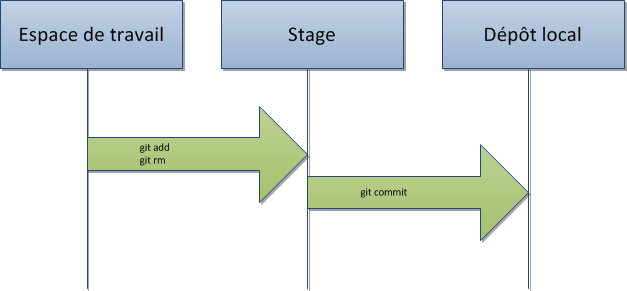
\includegraphics[width=\textwidth]{./images/staging-area.png}
  \end{center}
  Dans git, \alert{commit} a le sens de \textit{coucher par écrit} ou
\textit{acter}.
\end{frame}
%-------------------------------------------------------------------------------

\begin{frame}[fragile]\frametitle{TP : git clone, git log}
  Cloner un projet simple et regarder les commits / logs.
  \note{pas de push, on verra ça dans la partie 2 : avec un seul remote, les
conflits sont inévitables}
\end{frame}
\begin{frame}[fragile]\frametitle{TP : lifecycle simple}
  git init
  add, reset HEAD, commit, rm, etc
  % TODO : schema sur les differents etats des modifs, avec les commandes
\end{frame}
% max 80 columns : merges become messy with pure text and longer lines.
% vim: set colorcolumn=+1 textwidth=80:
